\section{Radiation Processes in Gamma-ray Astrophysics}

Nonthermal radiation observed from astrophysical sources is
typically believed to originate in syncrotron \ac{IC}, and the
decay of neutral \pion particles.  We will discuss these processes
in \subsecref{synchrotron}, \subsecref{inverse_compton}, and
\subsecref{bremsstrahlung} respectively.

\subsection{Synchrotron}
\subseclabel{synchrotron}

\begin{figure}[htbp]
  \centering 
    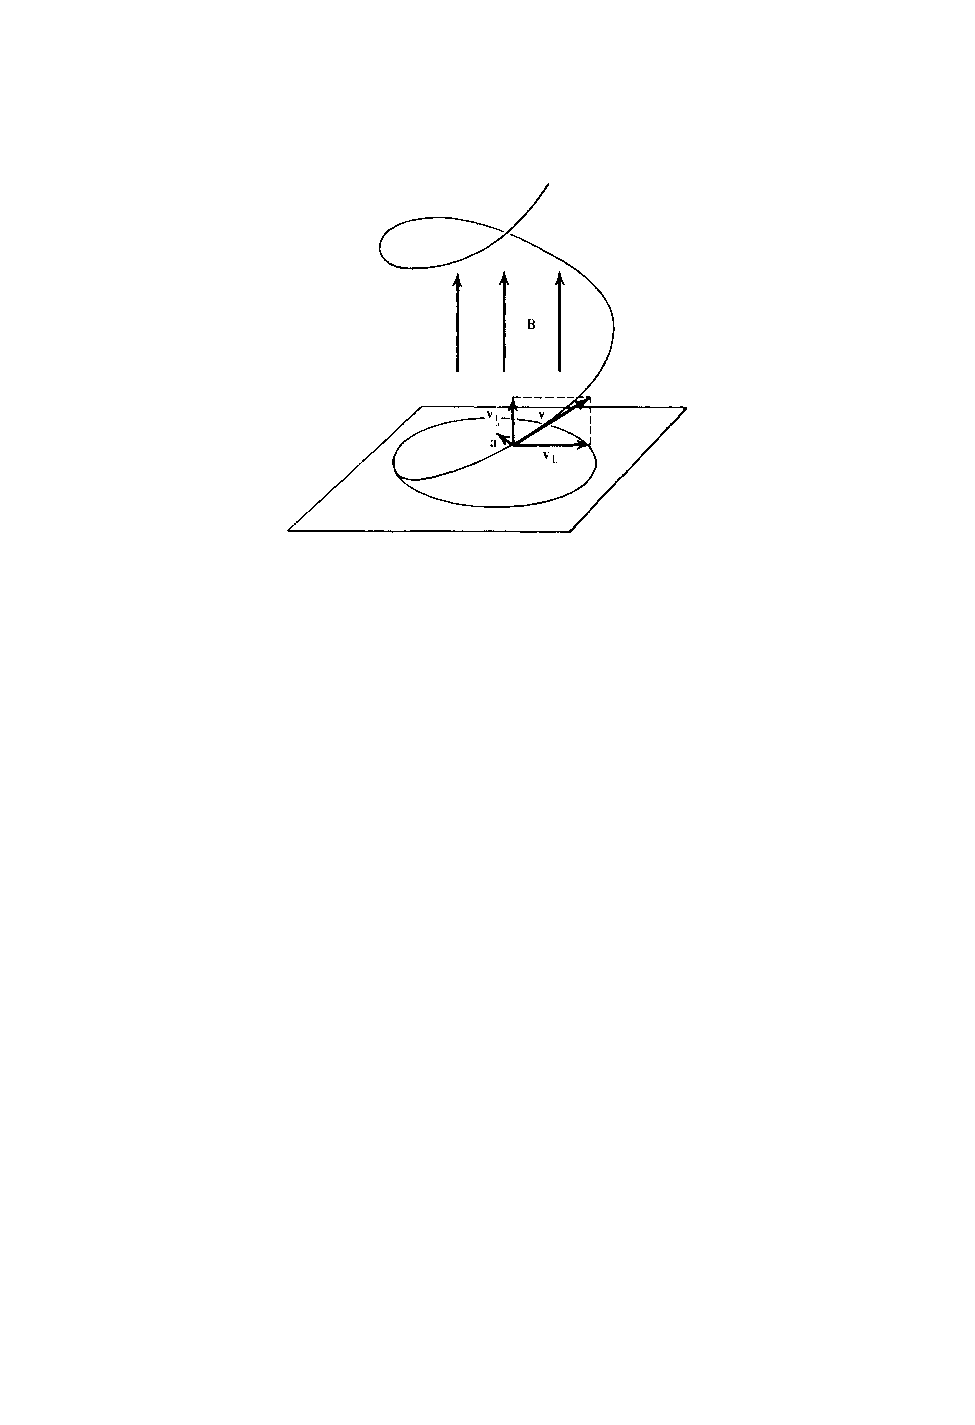
\includegraphics{chapters/introduction/figures/syncrotron_radiation_spiral.pdf}
    \caption{In synchrotron radiation, charged particles spiral along
      magnetic filed lines, radiating photons as they accelerate.}
  \figlabel{syncrotron_radiation_spiral}
\end{figure}


The synchrotron radiation processes is commonly observed in
astrophysics. It is caused when charged particles, typically
electrons, spiral around magnetic field lines.  As they
accelerate, they radiate photons.  This process is illustrated in
\figref{syncrotron_radiation_spiral}.
This emission is discussed thoroughly in
\cite{blumenthal_1970a_bremsstrahlung-synchrotron} and
\cite{rybicki_1979a_radiative-processes}.
In what follows, we adopt the notation from
\cite{houck_2006a_models-nonthermal}.

A charged particle of 
mass $\mass$ and charge $\charge$ in a magnetic field
of strength 
\MagneticFieldVector
will experince an
electromagnetic force:
\begin{align}
% equation 6.1a in R&L 1979
  \dbydt (\gamma m \VelocityVector) = & \frac{q}{c} \cross{\VelocityVector}{\MagneticFieldVector}
\end{align}
This force will cause a particle to accelerate around
the magnetic field lines, causing it
to radiate by maxwell's equations.

The power emitted at a frequency $\frequency$ 
by particle spiraling will be
\begin{equation}
% equation 6.33 in R&L 1979
  \eqnlabel{power_emitted_particle_sync}
  \power_\text{emitted}(\frequency) = 
  \frac{\sqrt{3} \charge^3 B \sin\alpha}{\mass \speedoflight^2} F(\frequency/\frequency_c)
\end{equation}
where $\alpha$ is the angle between the particle's velocity vector and
magnetic field vector.
Here,
% equation 6.31c in R&L 1979
\begin{equation}
  F(x) \equiv x \int_x^\infty K_{\tfrac{5}{3}} (\xi) d\xi,
\end{equation}
and
\begin{equation}
  \eqnlabel{characteristic_freqnecy_synctotron}
% equation 6.11a in R&L 1979
\frequency_c = \frac{3q \MagneticField \gamma^2}{4\pi \mass \speedoflight} 
\sin\alpha \equiv \nu_0 \gamma^2 \sin\alpha
\end{equation}

Because power is inversely-proportional to mass, synchotron radiation
is almost always assumed to come from electrons.

Now, we assume a population of particles and compute the total
emission. We say that $\ParticleDistribution(\momentum,\alpha)$ is the number of particles
per unit momentum and solid angle with a momentum $\momentum$ and
pitch angle $\alpha$.

We find the total power emitted by integrating over particle
momentum and distribution
\begin{equation}
  \frac{\derivative W}{\derivative\time}=
  \int \derivative \momentum 
  \int \derivative \solidangle
  \power_\text{emitted}(\frequency)
  \ParticleDistribution(\momentum,\alpha)
\end{equation}
If we assume the pitch angles of the particles to be isotropically
distributed and include \eqnref{power_emitted_particle_sync}, we
find that the photon emission per unit energy and time is
\begin{equation}
  \frac{\derivative \ParticleDistribution}{\derivative \omega \derivative \time} =
  \frac{\sqrt{3}q^3 B}{h m_e c^2 \angularfrequency}
  \int \derivative\momentum
  \ParticleDistribution(\momentum)
  R \left(\frac{\omega}{\omega_0 \gamma^2}\right)
\end{equation}
where
\begin{equation}
  R(x) \equiv \frac{1}{2} \int_0^\pi
  \derivative \alpha \sin^2 \alpha
  F\left(\frac{x}{\sin\alpha}\right)
\end{equation}

It is typical in astrophysics to assume a 
a power-law distribution of electrons written as
\begin{equation}
% equation 6.20a in R&L 1979
\eqnlabel{ElectronPowerLawEnergyDistribution}
  \ParticleDistribution(\momentum) \derivative\momentum = 
  \kappa \momentum^{-\spectralindex} \derivative\momentum.
\end{equation}
For a powerlaw distribution of photons integrated over
pitch angle, we find
\begin{equation}
\TotalPower(\angularfrequency) \propto \kappa \MagneticField^{(p+1)/2} 
\angularfrequency^{-(p-1)/2}.
\end{equation}
See, \cite{rybicki_1979a_radiative-processes} 
or \cite{longair_2013a_energy-astrophysics} for a full derivation.
This shows that, assuming a power-law electron distribution,
the electron spectral index can be related to the photon spectral
index.

\subsection{\Actitle{IC}}
\subseclabel{inverse_compton}

Normal compoton scattering involves a photon colliding with a free electron
and transfering energy to it. In \ac{IC} scattering, a high-energy 
electron interacts with a low-energy photon imparting energy to it.
This process occurs when highly-energetic electrons interact with
a dense photon field.

The derivation of \Ac{IC} emission requires a quantum
electrodynamical treatment. It was first computed in
\cite{klein_1929a_streuung-strahlung}, and the derivation is described
in \cite{blumenthal_1970a_bremsstrahlung-synchrotron}.  In what follows, we follow
the notational convetion of \cite{houck_2006a_models-nonthermal}.

We assume a population of relativistic ($\gamma\gg1$) electrons
written as $\ParticleDistribution(\momentum)$ which is contained inside isotropic 
photon distribution with number density $n(\omega_i)$.

The distribution of photons 
emitted by \ac{IC} scatter is
written as
\begin{equation}
  \frac{\derivative\ParticleDistribution}{\derivative\omega\derivative\time} = 
  c \int d \omega_i n(\omega_i)
  \int_{p_\text{min}}^\infty  dp
  \ParticleDistribution(p) 
 \KleinNishinaCrossSection(\gamma,\omega_i,\omega)
\end{equation}
where $\omega$ is the outgoing photon energy written
in units of the electron rest mass energy, $\omega\equiv h\nu/(m_e c^2)$,
and $\KleinNishinaCrossSection$ is the Klein-Nishina cross section.

The Klein-Nishina cross section is
\begin{equation}
\KleinNishinaCrossSection(\gamma,\omega_i,\omega) = \frac{2\pi r_0^2}{\omega_i \gamma^2}
  \left[
  1 + q - 2q^2 + 2q\ln q + \frac{\tau^2 q^2 (1-q)}{2(1+\tau q)}
  \right]
\end{equation}
Here,
\begin{equation}
  q \equiv \frac{\omega}{4 \omega_i \gamma (\gamma-\omega)},
\end{equation}
$\tau \equiv 4\omega_i \gamma$, and $r_0 = e^2/(m_e c^2)$ is the classical
electron radius.
The threshold electron lorentz factor is
\begin{equation}
  \gamma_\text{min} =
  \frac{1}{2} 
  \left(
  \omega + \sqrt{\omega^2 + \frac{\omega}{\omega_i}}
  \right)
\end{equation}

Typically, \ac{IC} emision is assumed to originate when
a power-law distribution of electrons
(see \eqnref{ElectronPowerLawEnergyDistribution})
interacts with
a thermal photon distribution
\begin{equation}
  n(\omega_i) = 
  \frac{1}{\pi^2\lambda^3} 
  \frac{\omega_i^2}{e^{\omega_i/\Theta} -1}
\end{equation}
where $\lambda=\hbar/(m_e c)$ and $\Theta=kT/(m_e c^2)$.
Typically, \ac{IC} emission happens off CMB photons
with $T=2.725\unitspace\kelvin$.
We conclude by noting that the free-parameters of 
\ac{IC} emission are the the assumed particle spectrum
and photon field.

\subsection{Bremsstrahlung}
\subseclabel{bremsstrahlung}

Bremsstrahlung radiation is compoosed of electron-electron and electron-ion interactions.
In either case, 
we assume a 
differential spectrum of accelerated electrons $\ParticleDistribution_\electron(\energy)$ 
that interacts with a target density of electrons (\ElectronDensity) or ions (\IonDensity).

\begin{equation}
  \frac{\derivative \ParticleDistribution}{\derivative\energy\derivative\time} =
  \ElectronDensity \int \derivative\energy
  \ParticleDistribution_\electron(\energy) \velocity_\electron
  \frac{\derivative\CrossSection_{\electron\electron}}{\derivative\energy} +
  \IonDensity \int \denergy
  \ParticleDistribution_\electron(\energy) \velocity_\electron
  \frac{\derivative\CrossSection_{\electron\AtomicNumber}}{\derivative\energy}
\end{equation}

Here, $\velocity_\electron$ is the velocity of the
electron, and $\CrossSection_{\electron\electron}$ and
$\CrossSection_{\electron\AtomicNumber}$ are the electron-electron and
electron-ion cross sections.
The actual formulas for 
$\derivative\CrossSection_{\electron\electron}/\derivative\energy$
and 
$\derivative\CrossSection_{\electron\AtomicNumber}/\derivative\energy$
are quite involved.  The electron-electron cross section was worked out
in \cite{haug_1975a_bremsstrahlung-production}.  The electron-ion cross
section is called the The Bethe-Heitler cross-section and is worked
out in the Born approximation in \cite{heitler_1954a_quantum-theory}
and \cite{koch_1959a_bremsstrahlung-cross-section}.  A more
accurate relativisatic correction to this formula is given in
\cite{haug_1997a_nonrelativistic-bremsstrahlung}.  We refer
to \cite{houck_2006a_models-nonthermal} for a detailed numerical
implementation of these formulas.

\subsection{Pion Decay}

Neutral \pion decay occurs when highly-energetic protons interact with
thermal protons. This
emission happens when protons decay into neutral pions through $pp \processarrow
\pion + X$ and the $\pion$ subsequently decay through $\pion \processarrow 2\gamma$.
The gamma-ray emission from neutral pion decay can be computed
as
\begin{equation}
  \frac{\derivative\ParticleDistribution}{\derivative\energy\derivative\time} = 
  \HydrogenDensity \int \denergy \velocity_\proton \ParticleDistribution_\proton(\energy) 
  \frac{\derivative\CrossSection_{\proton\proton}}{\derivative\energy}
\end{equation}
Here, $\ParticleDistribution_\proton(\energy)$
is the differential proton distribution,
$\derivative\CrossSection_{\proton\proton}/\derivative\energy$
is $\gamma$-ray cross section through proton-proton interactions, and
$\HydrogenDensity$ is the target hydrogen density.  The computation
of $\derivative\CrossSection_{\proton\proton}/\derivative\energy$ is
rather invovled. Typically, people employ a parmaeteriztaion of 
a very detaield calcuation of the cross section 
from \cite{kamae_2006a_parameterization-gamma}.
